\documentclass{article}
\usepackage[utf8]{inputenc}
\usepackage[official]{eurosym}
\usepackage{graphicx}
\usepackage[font=small,labelfont=bf]{caption}

\begin{document}

The Iris dataset was chosen, because of its low dimensionality and its small number of samples, which fulfils the requirement to be contrary to the other selected set. Furthermore, it is a very well known dataset, which allows comparison and therefore gives feedback on the performance our results. In general, preprocessing is not mandatory, however since the dataset contains only rational data types, it would be interesting two compare the scaled data versus the non-scaled one. A selection of features is not necessary, since it only consists of four dimensions and already performs quite well.

\subsection{Characteristics}

\begin{itemize}
\item No missing values
\item 3 different target classes
\item Rational quantities, e.g. sepal length, sepal width, petal length, petal width
\item 5 attributes
\item 150 samples
\end{itemize}

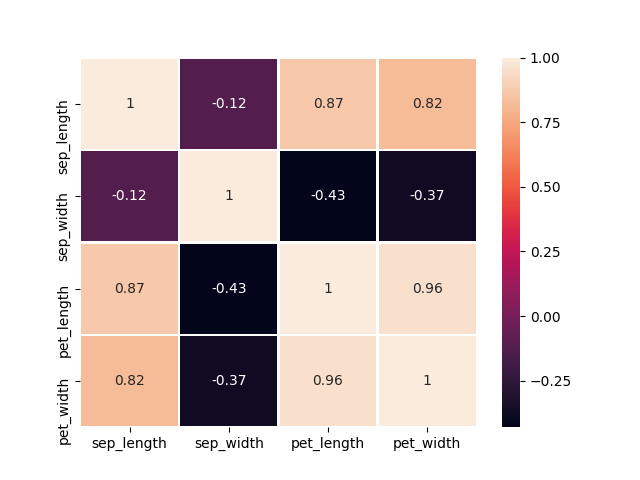
\includegraphics[width=\textwidth]{plots/heatmap.png}
\captionof{figure}{Heatmap of the different attrbutes of the Iris dataset}

\subsection{Characteristics of Classifiers}

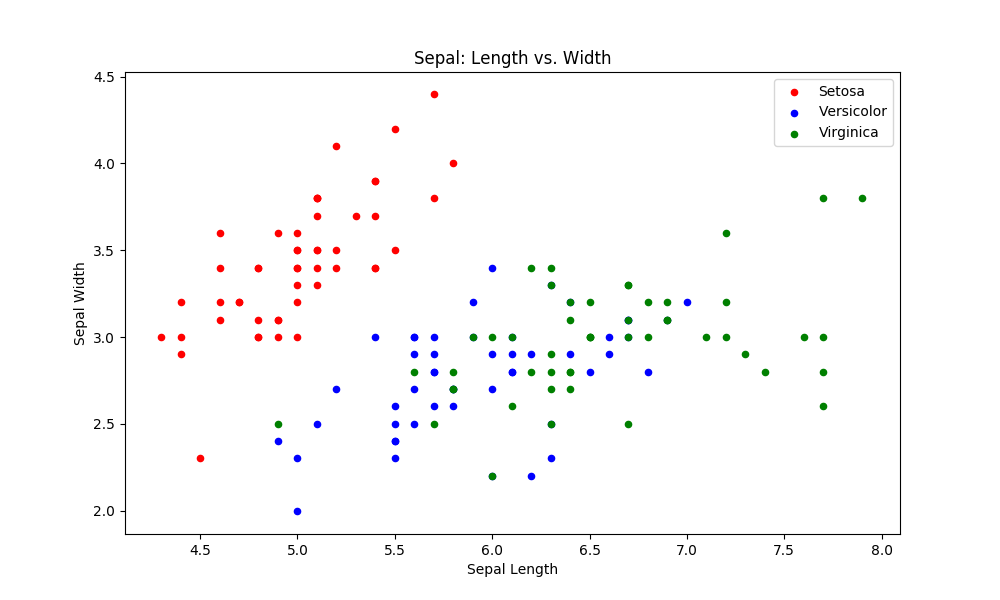
\includegraphics[width=\textwidth]{plots/sepal.png}
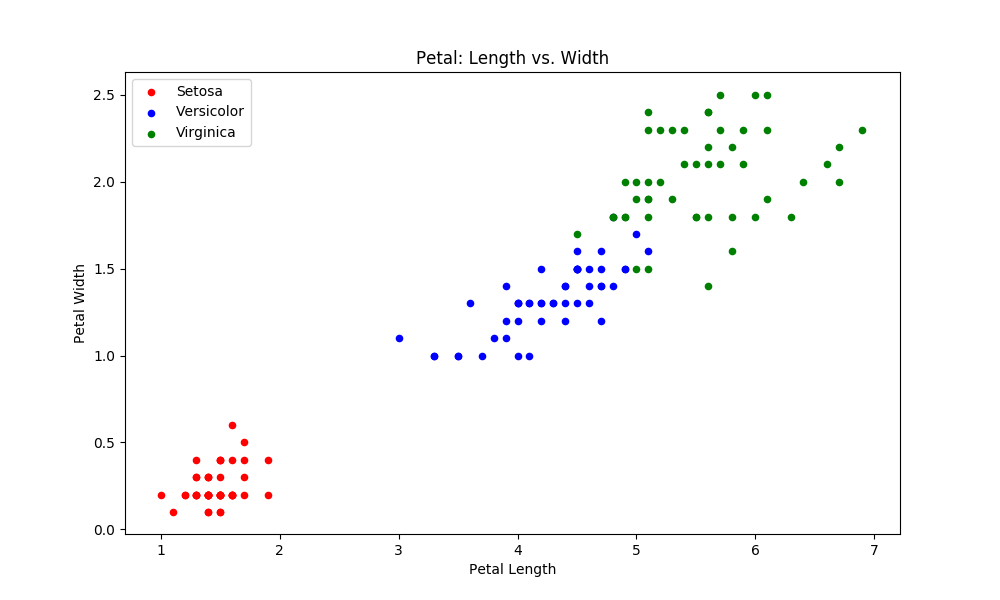
\includegraphics[width=\textwidth]{plots/petal.png}

\subsection{K Nearest Neighbours Classifier}

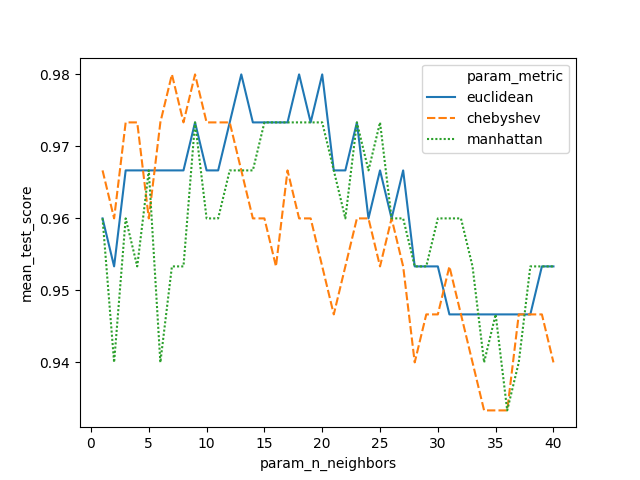
\includegraphics[width=\textwidth]{plots/knn_np_comparision.png}
\captionof{figure}{K Nearest Neighbours with different distance metrics}

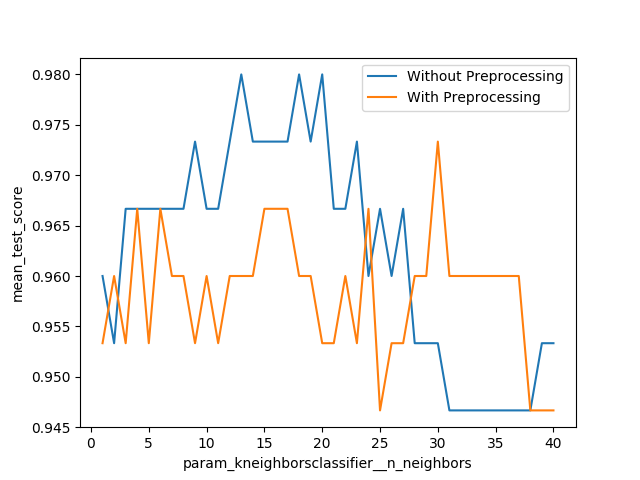
\includegraphics[width=\textwidth]{plots/knn_np_p_comparision.png}
\captionof{figure}{Preprocessing versus No-Preprocessing}

\subsection{Random Forest Classifier}
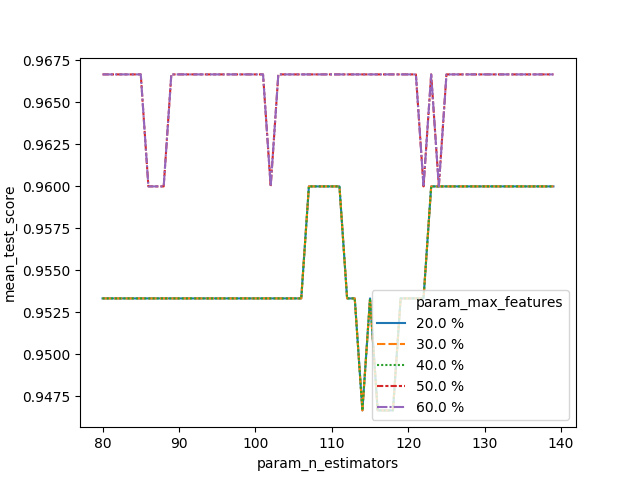
\includegraphics[width=\textwidth]{plots/rf_np_comparision.png}
\captionof{figure}{Comparison of the \textit{max\_features} attribute for different \textit{n\_estimators}}

\subsection{Multi-Layer Perceptron Classifier}
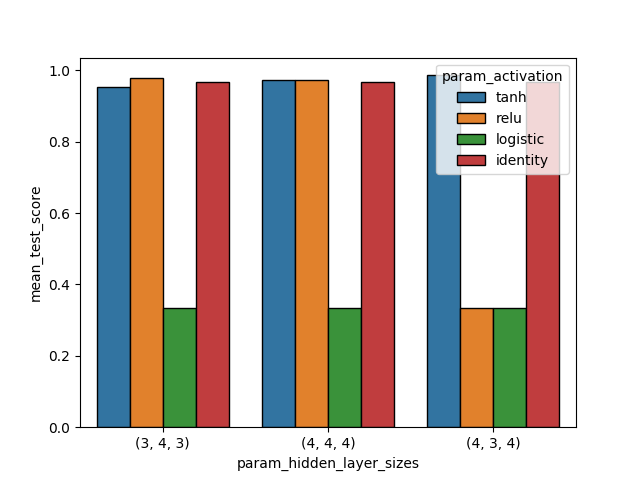
\includegraphics[width=\textwidth]{plots/mlp_np_comparision.png}
\captionof{figure}{Comparison of different models and activation functions}

\subsection{Conclusion}

\begin{table}[]
\begin{center}
\begin{tabular}{|l|l|l|}
\hline
                       & Preprocessing & No-Preprocessing \\ \hline
KNeighborsClassifier   & 0.9733        & 0.9800           \\ \hline
RandomForestClassifier & 0.9666        & 0.9666           \\ \hline
MLPClassifier          & 0.9666        & 0.9866           \\ \hline
\end{tabular}
\caption{Comparision of accuracy of different techniques with- and without preprocessing}
\end{center}
\end{table}

\begin{table}[]
\begin{center}
\begin{tabular}{|l|l|l|}
\hline
                       & Holdout & Cross Validation \\ \hline
KNeighborsClassifier   & 0.9333  & 0.9800           \\ \hline
RandomForestClassifier & 0.9666  & 0.9666           \\ \hline
MLPClassifier          & 1.0000  & 0.9866           \\ \hline
\end{tabular}
\caption{Comparision of accuracy of holdout versus cross-validation}
\end{center}
\end{table}
\begin{table}[]
\begin{center}
\begin{tabular}{|l|l|l|l|l|l|}
\hline
                       & Accuracy & Precision & Recall & F1     & Runtime (sec) \\ \hline
KNeighborsClassifier   & 0.9800   & 0.0.9833  & 0.9799 & 0.9797 & 0.0034        \\ \hline
RandomForestClassifier & 0.9600   & 0.9644    & 0.9600 & 0.9597 & 0.1947        \\ \hline
MLPClassifier          & 0.9800   & 0.9848    & 0.9800 & 0.9793 & 1.5557        \\ \hline
\end{tabular}
\caption{Comparision of different performance metrics and runtimes}
\end{center}
\end{table}

\end{document}